% Mirror: https://github.com/SIGma-UIUC/presentation-format
% --------------------------------------------------------------------
% This is a simple Beamer document that uses beamerthemesigma.sty
% Reading the comments should help you create a presentation even if
% you've never used Beamer before.
% --------------------------------------------------------------------

% Set our document class to Beamer
\documentclass[aspectratio=169]{beamer}
% \documentclass[aspectratio=169, handout]{beamer}
% Add handout option to ignore pauses

% From Jeff E
\usepackage{algo}
% Some more macros
\usepackage{sigmastyle}


% Set a title
\title{Introduction to Qubits}

% Set a subtitle if you desire

% Whoever worked on the presentation:
\author{Parth Deshmukh, Andrey Vlasov}

% Date looks ugly, so leave blank
\date{}
\newcommand{\twovec}[2]{\begin{pmatrix} #1 \\ #2 \end{pmatrix}}
\newcommand{\tworvec}[2]{\begin{pmatrix} #1 & #2 \end{pmatrix}}

% An institute name, if you're so inclined
% \institute{University of Illinois Urbana-Champaign}

% Use the SIGma theme for this Beamer presentation
\usetheme{sigma}
% --------------------------------------------------------------------

% Begin document
\begin{document}

% Beamer calls each slide a "frame", defined within the environment:
% \begin{frame}
%   <frame content here>
% \end{frame}

% This frame is just the title.
\begin{frame}
\titlepage
\end{frame}

\begin{frame}{Parth}
    \begin{itemize}
        \item Senior in Mathematics
        \item Main interests: Algebra, Logic, Econometrics, Combinatorics
        \item Vice President of MATRIX
        \item Coffee Club
    \end{itemize}
\end{frame}

\begin{frame}{Andrey}
    \begin{itemize}
        \item Freshman in Mathematics
        \item Main interests: Math, Quantum Computing, Entrepreneurship, Quantitative Finance
        \item Zero2One Startup Incubator
        \item Tutoring Startup
    \end{itemize}
\end{frame}

\begin{frame}{MATRIX}
    \begin{itemize}
        \item We've got two events this week - free pizza and snacks at both!
        \item On the ruler and compass problem: tomorrow, Oct 3rd, 6:30pm in 1051 Lincoln Hall
        \item Trivia Night: Thursday, Oct 5th, 6:30pm in 1022 Lincoln Hall
        \item Scan the QR code for our Discord
    \end{itemize}
    \begin{figure}[h]
        \centering
        
\includegraphics[scale=0.15]{qrcode.png}
    \end{figure}
\end{frame}
% A frame with the table of contents.
% This frame's title is "Outline".
\begin{frame}{Outline}
  \tableofcontents
\end{frame}

\begin{frame}{Important notes}
  % Let's put some real content in this frame:
  \begin{itemize}
    \item This is part 1 of 2 in a series on quantum error correction. Make sure to come to the next one!
    \item Some advice: when learning quantum mechanics, treat it like a game with rules to play. (Unless you're a physicist.)
  \end{itemize}
\end{frame}

% Start a section: *sections* (subsections, etc.) are what show up in the TOC.
\section{What is a qubit?}
% Section pages can be printed thus:
\frame{\sectionpage}
% There's a way to automate this, see:
% https://tex.stackexchange.com/questions/178800/creating-sections-each-with-title-pages-in-beamers-slides/178803

\begin{frame}{Classical versus Quantum Bits}
    \begin{itemize}
        \item A classical bit can be either 0 or 1
        \item Quantum bits (qubits) can be 0, 1, or a superposition of the two \pause
        \item What does that mean \textit{mathematically}?
    \end{itemize}
\end{frame}

\begin{frame}
  \frametitle{Qubits, Formally}
  \begin{itemize}
      \item A qubit is represented by a \textcolor{sigma@mainblue}{statevector} in a \textcolor{sigma@mainblue}{state space} \pause
      \item The state space is a \textit{Hilbert space}, aka $\mathbb{C}^k$ \pause
      \begin{itemize}
          \item There are other Hilbert spaces, but we only really need $\mathbb{C}^k$
          \item Hilbert spaces have inner products and associated norms that make it a complete metric space: these are linear algebra concepts you don't need to understand, but the point is having these makes everything nicer
      \end{itemize} \pause
      \item A statevector is simply a unit (norm 1) vector of the state space \pause
      \item Examples: $|0 \rangle = \twovec{1}{0}, |1\rangle = \twovec{0}{1}, |+\rangle = \frac{1}{\sqrt{2}}\twovec{1}{1}, |i\rangle = \frac{1}{\sqrt{2}}\twovec{1}{-i}$
  \end{itemize}
\end{frame}

% Use \pause to make stuff readable
% Large walls of text scare the audience, we don't want that
% Introducing stuff sequentially allows for questions
\begin{frame}{What was that notation!?}
    \begin{itemize}
        \item Quantum mechanics uses \textcolor{sigma@mainblue}{bra-ket notation} \pause
        \item $|\phi \rangle$ (a "ket") is a vector, $\langle \phi |$ (a "bra") is its conjugate transpose \pause
        \begin{itemize}
            \item Example: $|0\rangle = \twovec{1}{0}, \langle 0 | = \tworvec{1}{0}$ or $|\chi\rangle = \twovec{0}{i}, \langle \chi | = \tworvec{0}{-i}$
        \end{itemize} \pause
        \item Putting the two together: $\langle \phi | \psi \rangle$ is the inner product of $| \phi \rangle$ and $| \psi \rangle$ \pause
        \item Examples:
        \begin{itemize}
            \item $\langle \chi | 0 \rangle = (1*0) + (0 * i) = 0$ \pause
            \item $\langle \chi | \chi \rangle = (0*0) + (-i * i) = 1$
        \end{itemize}
    \end{itemize}
\end{frame}

\begin{frame}{More notation}
\framesubtitle{I promise it'll be over soon}
    \begin{itemize}
        \item $|0\rangle$ and $|1\rangle$ are an orthonormal basis over $\mathbb{C}^2$; by convention, we denote this the \textcolor{sigma@mainblue}{computational basis} \pause
        \begin{itemize}
            \item We could use any orthonormal basis! There's nothing special about $\{|0\rangle, |1\rangle\}$ versus the other ONBs except that it's the easiest to write down
        \end{itemize} \pause
        \item An arbitrary statevector $|\psi\rangle = \alpha|0\rangle + \beta|1\rangle = \twovec{\alpha}{\beta}$ \pause
        \item Recall we said statevectors have unit length; in other words, $\langle \psi | \psi \rangle = 1$ \pause
        \item Exercise: $\langle \psi | \psi \rangle = 1$ enforces conditions on $\alpha$ and $\beta$. What are they?
    \end{itemize}
\end{frame}

\section{Measuring and representing qubit states}

\begin{frame}{Quantum measurement}
    \begin{itemize}
        \item So how do we work with qubit states? \pause
        \item Measurement principle: we cannot directly get the statevector $|\psi \rangle$ of some quantum state. Measuring the state changes it! \pause
        \item We have to \textit{measure} it, collapsing it to one of two vectors in some basis (the computational basis, usually) \pause
        \item To measure $|\psi \rangle,$ take the dot products: $\langle \psi | 0 \rangle ^2$ is the probability it collapses to 0, and $\langle \psi | 1 \rangle ^2$ is the probability it collapses to 1 \pause
        \item \textcolor{sigma@alertred}{Exercise:} Find the probabilities of $|\psi \rangle = \alpha|0\rangle + \beta|1\rangle$ collapsing to 0 or 1
    \end{itemize}
\end{frame}

\begin{frame}{Representing statevectors}
    \begin{itemize}
        \item By definition, a statevector has norm 1 \pause
        \item This leads to a geometrical intuition of what a statevector looks like \pause
        \item In two dimensions, we can represent all vectors of norm 1 with a unit circle \pause
        \item In quantum mechanics, we represent 3D statevectors using a unit sphere
    \end{itemize}
\end{frame}

\begin{frame}{The Bloch Sphere}
    \begin{figure}
        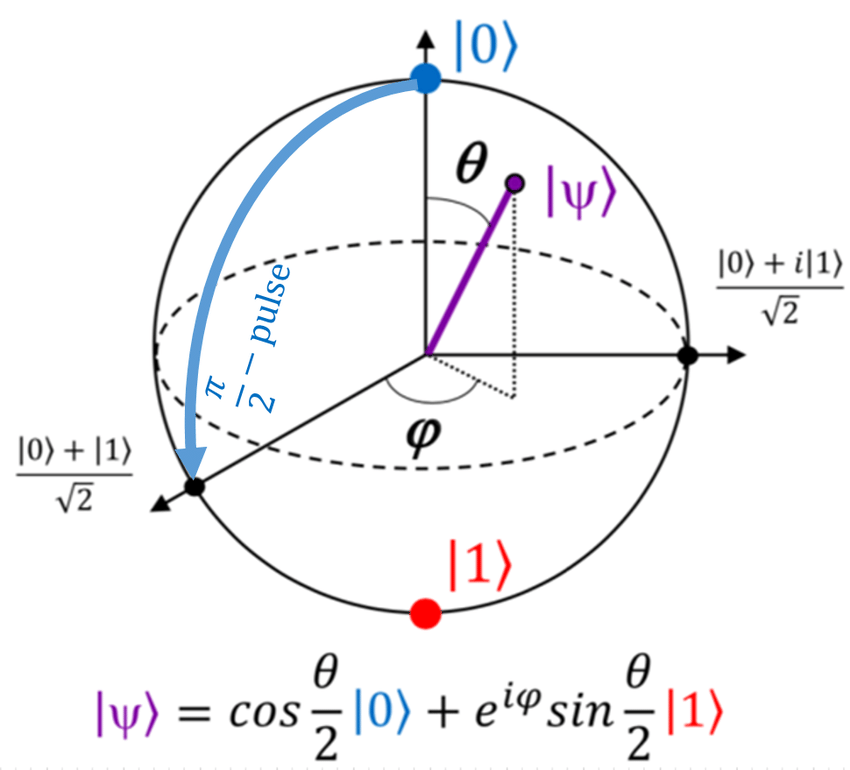
\includegraphics[width=8cm]{Bloch.png}
    \end{figure}
\end{frame}

\begin{frame}{The Bloch Sphere}
    \begin{itemize}
        \item Recall that an arbitrary statevector $|\psi\rangle = \alpha|0\rangle + \beta|1\rangle$ is a superposition of the two states $|0\rangle$ and $|1\rangle$ chosen as our ONB \pause
        \item Thus, a qubit can be any point on the Bloch sphere if we properly choose $\alpha$ and $\beta$ \pause
        \item We do so by letting $\alpha = \cos{\frac{\theta}{2}}$ and $\beta = e^{i\phi}\sin{\frac{\theta}{2}}$, so that $\theta$ is the polar angle and $\phi$ is the azimuthal angle \pause
        \item We now have a system of polar coordinates for describing statevectors of a qubit \pause
        \item Just like with wavefunctions, the squared norms $|\alpha|^2$ and $|\beta|^2$ describe the probability of the qubit collapsing into either of our two basis states
    \end{itemize}
\end{frame}

\begin{frame}{Back to Reality}
\framesubtitle{How does this relate to actual qubits?}
\begin{itemize}
    \item Physical qubits are things like electrons or photons, which have certain properties that are described via quantum states, e.g. the spin of an electron \pause
    \item We need the mathematics of quantum mechanics to be able to describe these qubits, and how we can mess with them \pause
    \item The statevector tracks the quantum state of a physical qubit \pause
    \item Our allowed operations are matrices that don't change the length of a vector: the \textcolor{sigma@mainblue}{special unitary group SU(n)} \pause
    \begin{itemize}
        \item Spoiler: quantum gates are exactly these matrices!
    \end{itemize}
\end{itemize}
\end{frame}

\section{Qubit errors and why it's so hard to correct them}
% Section pages can be printed thus:
\frame{\sectionpage}

\begin{frame}{What is an error?}
    \begin{itemize}
        \item In classical computing, an error on a bit flips that bit \pause
        \item In quantum computing, a qubit can be in an infinite number of positions! \pause
        \item An error is \textit{any} perturbation of a qubit's state \pause
        \item $|0\rangle$ could become $|1\rangle$ or $|+\rangle$, or with a smaller perturbation, $\frac{1}{\sqrt{6}}\twovec{5}{1}$
    \end{itemize}
\end{frame}

\begin{frame}{Errors on the Bloch Sphere}
    \begin{itemize}
        \item Infinitely many positions on the Bloch Sphere mean infinitely many possible errors! \pause
        \item In real quantum computers, small interactions with the environment can cause the qubit to "drift" on the Bloch Sphere \pause
        \item A \textit{partial bit flip error} rotates the statevector about the $x$-axis
        \item A \textit{phase flip error} rotates the statevector about the $z$-axis \pause
        \item We want to find a way to correct both types of errors
    \end{itemize}
\end{frame}

\section{Fixing errors (?)}

\begin{frame}{So how do we fix an error?}
    \begin{itemize}
        \item An easy classical method is called a \textcolor{sigma@mainblue}{repetition code} \pause
        \item Add redundancy to a bit: 0 becomes 000 \pause
        \item If any one bit flips, we can spot it and fix it \pause
        \item To protect against two bit flips, have four bits of redundancy: 0 becomes 00000 \pause
        \item \textcolor{sigma@alertred}{Exercise:} how many bits of redundancy do we need to protect against $n$ bit flips?
    \end{itemize}
\end{frame}

\begin{frame}{Redundancy for qubits}
    \begin{itemize}
        \item So we just need to add redundant qubits, right? \pause
        \item Nope. There's an important theorem called the \textcolor{sigma@mainblue}{no-cloning theorem:} 
    \end{itemize} \pause
    \begin{thrm}
        If $|\psi \rangle$ is an arbitrary quantum state, we cannot make a copy of it. That is, we cannot go from $|\psi \rangle |0\rangle \rightarrow |\psi \rangle |\psi \rangle.$
    \end{thrm}
    \begin{itemize} \pause
    \item Note: $|\psi\rangle |0\rangle$ is the \textcolor{sigma@mainblue}{tensor product} of $|\psi\rangle$ and $|0\rangle$; we represent multiple qubits in a system by taking their tensor product \pause
    \item The no-cloning theorem rules out repetition codes entirely \pause
    \item Sketch of proof: if we want to duplicate a state $|\psi\rangle = \alpha|0\rangle + \beta|1\rangle,$ we need to know $\alpha$ and $\beta$. But we can't measure them!
    \end{itemize}
\end{frame}

\begin{frame}{Conclusion}
    \begin{itemize}
        \item No-cloning theorem rules out basic error correction schemes \pause
        \item We need something more sophisticated \pause
        \item There are classical error correcting codes, that instead of using redundancy, use \textit{parity bits} \pause
        \item We'll use a similar idea, indirectly checking the qubits to make a bit-flip code. To be covered next week!
    \end{itemize}
\end{frame}

% However, this doesn't work in math mode. It is quite annoying to figure out
% So just copy this as reference
% This works for \onslide<> and \item<>
% Really good read on this: 
%   https://www.texdev.net/2014/01/17/the-beamer-slide-overlay-concept/
%%% \begin{frame}{Sequential Math Frames}
%%%     Here is a sentence \pause
%%%     
%%%     I shall now carry out some calculations \pause
%%%     \begin{align*}
%%%         \onslide<+->{\zeta(s) &= \sum_{n = 1}^\infty %%% \frac{1}{n^s} \\}
%%%         \onslide<+->{&= \prod_{p \in \text{primes}} \frac{1}{1 %%% - p^{-s}} \\}
%%%         \onslide<.->{&= \frac{1}{1 - 2^-s} \cdot \frac{1}{1 - %%% 3^-s} \cdots \\}
%%%         \onslide<+->{&= \frac{1}{\Gamma(s)} \int_0^\infty %%% \frac{x^{s - 1}}{e^x - 1} ~\textrm{d}x\\}
%%%     \end{align*}
%%% \end{frame}

% Quotes are fun, find some to use!
\font\eightss=cmssq8
\font\eightssi=cmssqi8
\newcommand\quoteAuthorDate[3]{\begingroup
  \baselineskip 10pt
  \parfillskip 0pt
  \interlinepenalty 10000 % not needed in example
  \leftskip 0pt plus 40pc minus \parindent
  \let\rm=\eightss
  \let\sl=\eightssi
  \everypar{\sl}#1\par
  \nobreak\smallskip
  \noindent\rm--- #2\unskip\enspace(#3)\par
  \endgroup}
% If someone can figure out how to horizontally center this and make the text bigger that'd be cool
\begin{frame}
    \begin{center}
        \item \quoteAuthorDate{To imagine the quantum spin of a particle, imagine a spinning ball, except it's not a ball and it's not spinning.}{John Physics}{\textcolor{sigma@mainblue}{1000 BC}}
    \end{center}
\end{frame}

% Remove this slide if you came up with all the material yourself
\begin{frame}{Bibliography}
    \nocite{wong2022introduction}
    \bibliography{refs}
    \bibliographystyle{alpha}
\end{frame}

\end{document}